\documentclass[a4paper]{article}

%% Language and font encodings
\usepackage[english]{babel}
\usepackage[utf8x]{inputenc}
\usepackage[T1]{fontenc}
\usepackage{setspace}
\usepackage{graphicx}
\usepackage{caption}
\usepackage{subcaption}
\usepackage{wrapfig}
\usepackage[labelfont=bf]{caption}
\usepackage{multicol}
\setlength{\columnsep}{0.5cm}
%% Sets page size and margins
\usepackage[a4paper,top=3cm,bottom=3cm,left=3cm,right=3cm,marginparwidth=1.75cm]{geometry}



%% Useful packages
%\usepackage{gensymb}
\usepackage{amssymb}
\usepackage{amsmath}
\global\csname @topnum\endcsname 0
\global\csname @botnum\endcsname 0
%\usepackage{graphicx}
\usepackage[colorinlistoftodos]{todonotes}
\usepackage[colorlinks=true, allcolors=blue]{hyperref}
\graphicspath{ {figure/} }
%triplespacing

\title{Sensor Integration in Architectural Environment and Light Fixture Configuration Optimization}
\author{Abinav Chandar \and Joel Abraham \and Young Min Kim}
\date{August 2017}

\begin{document} \twocolumn
\maketitle
\section{Introduction}

We present a system to integrate hybrid information and processing into a unified platform and visualization.
A number of the state of the art technology, including but not limited to smart phones, autonomous driving, smart homes, IoT (internet of things) technology, and assisting robots, depend on different types of sensors and actuators attached to the system.
We are interested in creating a unifying platform incorporating the geometric constraints of the acting environment.
That is, given a CAD model of the environment that sensors and actuators are located, the context and additional information is efficiently integrated into a platform that contains pre-known information.
Especially, we are looking at an architectural environment using Autodek Revit, a popular BIM (Building Information Modeling) framework that stores different functional and geometric hierarchy of information.
Given the architectural model, our presented platform include multiple types of sensors, whose outputs are analyzed into the processing unit to visualize and control actuators based on the specific goal of task.

With the goal in mind, there are two specific tasks that we focused.
First, we demonstrated the integration of a CAD model with functional information with hardware (in Section~\ref{sec:hardware}).
We utilized existing coding platform of Revit with plug-in and Dynamo scripts and incorporate location, sensor readings and actuators, namely temperature sensors, light sensors, motion sensors, and motors and robots with Arduino board and Firefly software.

Second, among possible problems we can solve with the integrated platform, we present a light optimization (in Section~\ref{sec:optimization}).
Given the light distribution and LED controllers, we can design the configuration to create a uniform lighting on the pre-defined region.
The problem and optimization is presented with a simple example.


%\section{Previous Work}

\section{Set Up}
\label{sec:hardware}

In order to get the most accurate data from our model we developed a robust harmoniously integrated sensor control and visualization environent. This environent consists of three parts: the sensing component, the processing and visualization component with Dynamo and Revit visualization model and the control component an array of light fixtures controlled by Arduino micro-controllers. The sensing component allows for efficent data collection by equipping an autuonomous robot with photosensors and an Arduino UNO to relay live light readings to the processing system. The processing system takes in the live stream of data through Firefly via a firmata into Dynamo to create a target optimization model. Lastly the model writes data to the Arduino control environment to dim the LED or translate a row or column of LEDs in the x or y direction.
%\textbf{TODO: first give a short summary/list/or table to outline the components.}





The Arduino UNO is a microcontroller board based on the ATmega328P (datasheet). It has 14 digital input/output pins (of which 6 can be used as PWM outputs), 6 analog inputs, a 16 MHz quartz crystal, a USB connection, a power jack, an ICSP header and a reset button. In order to get readings from all the points in a given environment we used an autonomous robot that traversed from point to point to get live light readings using a photoresistor.

\begin{figure*}
    \centering
    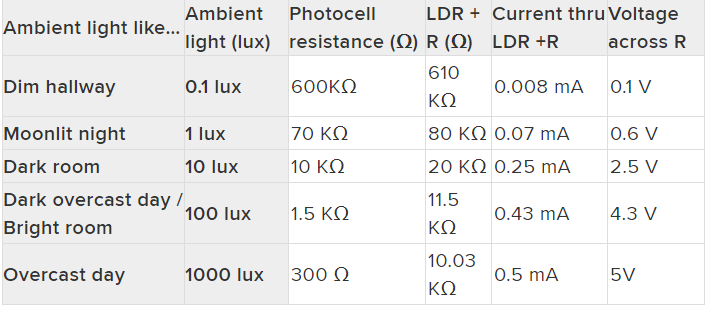
\includegraphics[width=0.9\textwidth]{Captureimg}
    \caption{Caption}-
    \label{fig:test}
\end{figure*}


A Photoresistor is a resistor that changes its resistive value (in ohms $\Omega$) depending on how much light is shining onto the sensor.The Resistance range: 200KΩ (dark) to 10KΩ (10 lux brightness) Sensitivity range: CdS cells respond to light between 400nm (violet) and 600nm (orange) wavelengths, peaking at about 520nm (green).
Power supply: pretty much anything up to 100V, uses less than 1mA of current on average (depends on power supply voltage) This Arduino UNO board communicates data through COM (communication) port 7. 



The Visualization and Optimization Model takes in data from Dynamo via Firefly and generates a visual model in Revit.
Open-source Dynamo is a visual programming extension for Autodesk® Revit that allows you to manipulate data, sculpt geometry, explore design options, automate processes, and create links between multiple applications. 
Firefly is a set of comprehensive software tools dedicated to bridging the gap between Dynamo- (a free plug-in for Revit) - the Arduino microcontroller and other input/output devices like web-cams, mobile phones, game controllers and more. It allows near real-time data flow between the digital and physical worlds – enabling the possibility to explore virtual and physical prototypes with unprecedented fluidity.
Every time the photocell senses it transmits that data through Firefly into Dynamo.

The Arduino UNO connects to Firefly using the Firefly firmata which is setup to read (digital and analog) values from the appropriate pins. So to get an actual reading from these sensors, you're sending and receiving signals very quickly on a standard digital pin. 

The Firefly firmata simply tells the Arduino UNO micro-controller to do a digital read. As  live data streams from the Arduino UNO sensing environment to the Dynamo Model we apply the Light Configuration Optimization algorithm (in Section~\ref{sec:optimization}).

The control system platform is an array of bright white LEDs connected to servos for movement in the x and y direction. In order to reach the target optimization model the control environment can dim individual LEDs move a row of LEDs in the x or y direction to deliver as uniform as possible lighting.This system is controlled by an Arduino UNO using COM port 4. 

Once the Dynamo model creates a target optimization model based on live light readings, Firefly will simply do a digitalwrite to the Arduino UNO COM 4. 


%\begin{figure*}
%    \centering
%    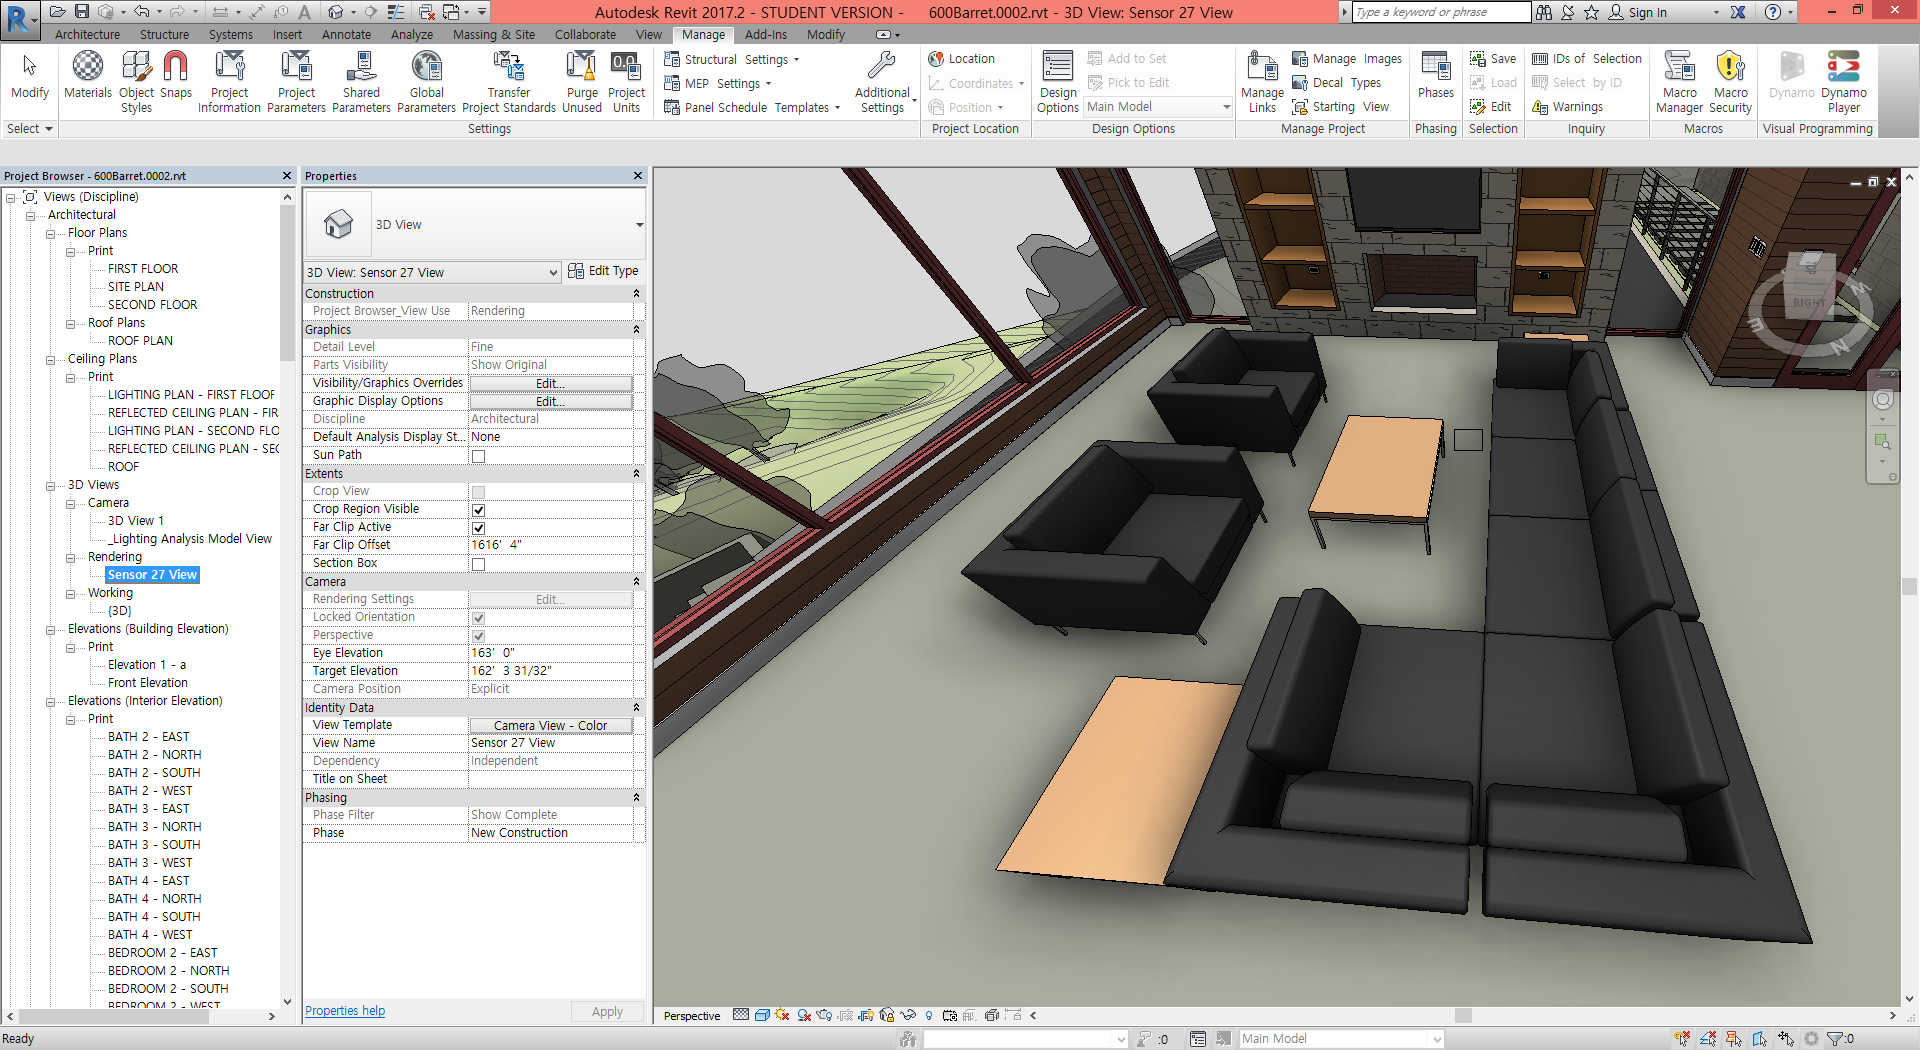
\includegraphics[width=0.9\textwidth]{camera27_capture}
%    \caption{Caption}
%    \label{fig:test}
%\end{figure*}

\section{Light Optimization}
\label{sec:optimization}
The problem of light optimization is presented as a representative example of our system's capabilities. Our optimization algorithm takes input data from the Arduino UNO sensors and directs the control system to modify the position and brightness of the LEDs accordingly. We will now formally introduce the problem of light optimization and discuss our solution.

Given an $M$ by $N$ target plane (X-Y plane) and a parallel source plane at a distance $Z$ from the target plane, we seek to find a configuration of $K$ LEDs on the source plane yielding maximally uniform light distribution on the target plane. A configuration of LEDs can be formally represented by a set of $k$ elements where each element is a 2-tuple consisting of an ordered pair, relating the integer-valued coordinates of the LED, and a brightness value, a non-negative real number no greater than 1. 

In order to formalize the goal of maximizing uniformity of light distribution, we model each LED as a Lambertian source. Under this model, the luminous intensity of an individual point LED is represented by Eq. (1) \cite{su}.
\begin{equation}
I(\theta) = I_0\cos^m (\theta_{1/2})
\end{equation}

Here, $\theta$ is the angle between the line segment connecting the target point and the LED. $\theta_{1/2}$ is the angular half-width, defined as the angle for which $I(\theta_{1/2}) = \frac{1}{2}I_0$. Since the angular half-width is provided by the manufacturer, we can solve Eq. (1) to define $m$, yielding Eq. (2) \cite{su}.
\begin{equation}
m = \frac{-\ln(2)}{\ln(\cos(\theta_{1/2}))}
\end{equation}
We define a target plane, to which the LEDs will be fixed, and a source plane, representing the area in which we seek to achieve a uniform light distribution. Since we can rewrite $cos(\theta)$ as $Z/d$ where $d$ is the distance between the target point and the LED, the luminous intensity at point $P = (X, Y, 0)$ contributed by a certain LED $Q = (x_q, y_q, Z)$ is given by Eq. (3) \cite{su}.

\begin{equation}
E(P, Q) = \frac{z^{m+1}I_{q,0}}{((X - x_q)^2 + (Y - y_q)^2 + Z^2)^{\frac{m+3}{2}}}
\end{equation}

Thus, given a set of LEDs, we can model the total irradiance at a point by summing Eq. (3) over all elements of the set. Eq. (4) \cite{su} yields the total irradiance at a single point in the target plane. 

\begin{equation}
E(X, Y) = \sum\limits_{q=1}^{K} \frac{z^{m+1}I_{q,0}}{((X - x_q)^2 + (Y - y_q)^2 + Z^2)^{\frac{m+3}{2}}}
\end{equation}

To best achieve a uniform light distribution, we define the cost function as $f: \mathbb{R}^K \rightarrow \mathbb{R}, f = \frac{\sigma}{\bar{E}}$ where $\sigma$ is the coefficient of variance root mean squared error given by Eq. (5), with $\bar{E}$ representing the average irradiance of all points in the target plane.  


\begin{equation}
\sigma = \frac{\sqrt{\sum\limits_{p=1}^{M*N}(E(x_p, y_p) - \bar{E})^2}}{M*N}
\end{equation}


Now, minimizing $f$ yields the LED configuration with maximum uniformity. Note that this objective function is non-convex, thus conventional optimization algorithms may prove inefficient for large values of $K, M,$ or $N$.

We tested various optimization techniques using a sample case with $M = N = k = Z = 5$. Initially, a complete space search was implemented, although it rapidly decreased in efficiency for $M$ and $N$ exceeding $8$. This approach iterated through every combination of $k$ points on the source plane and evaluated the cost of each configuration, yielding a complexity of $O({n \choose k}nk)$.

In order to account for cases for which the naive approach failed, we turned to simulated annealing, since it has been proven to be efficient for large search spaces. While our simulated annealing algorithm proved efficient, running in constant time, it often returned inaccurate solutions with a high error value. Various neighbor-finding algorithms were tested for simulated annealing, such as shifting points in a random direction by a fixed number of units and deleting one point at random and spawning a new one in a random location, although none demonstrated a significant increase in performance. 

\begin{figure}[b]
    \centering
    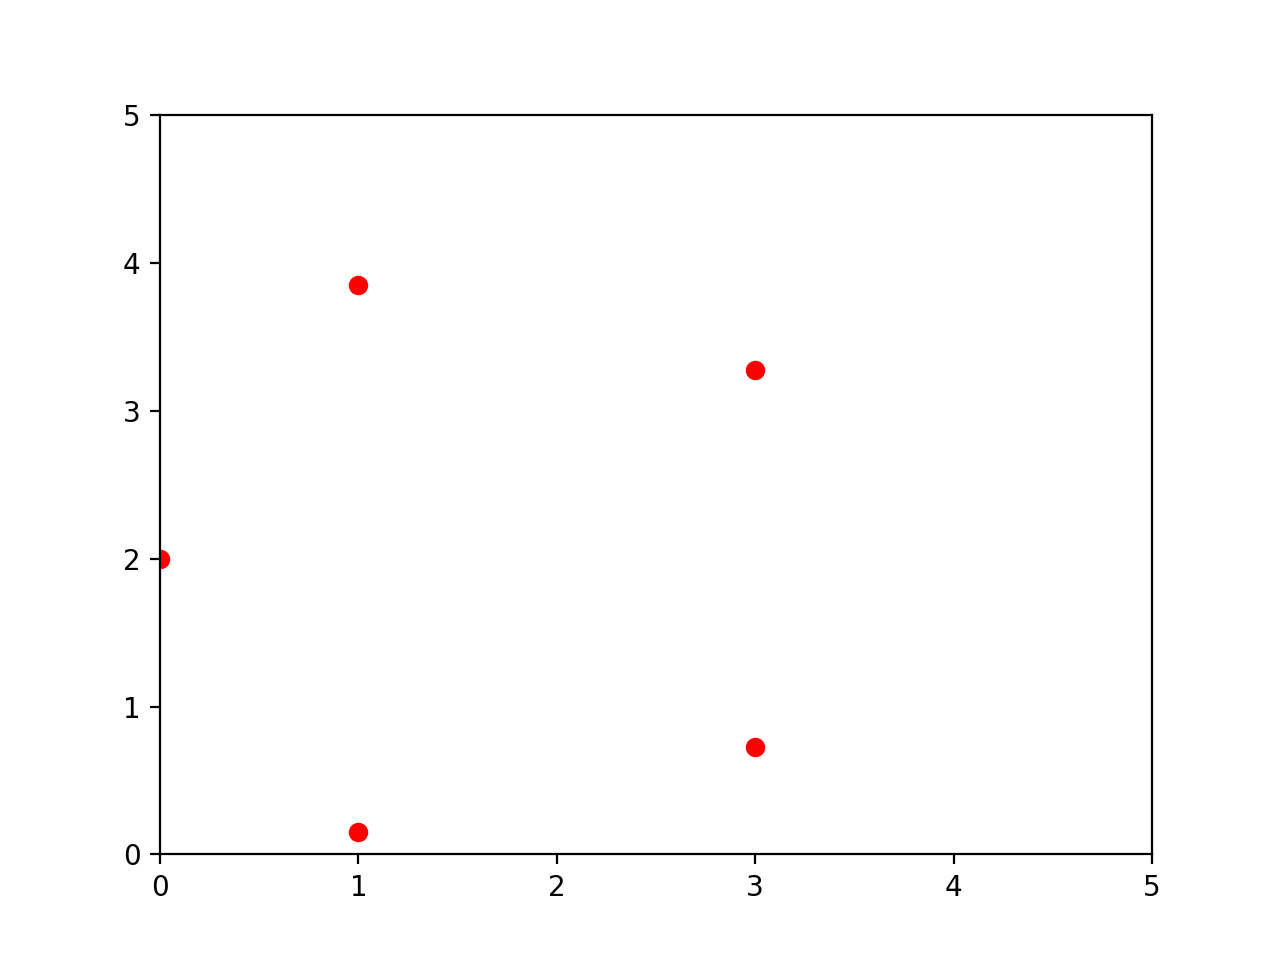
\includegraphics[width=0.5\textwidth]{Light_Optimization_L-BFGS}
    \caption{Optimal configuration of LEDs for M = N = k = Z = 5, yielding error value of 0.28}
    \label{solution}
\end{figure}

As such, we opted to use the SciPy (0.19.1) library for Python (3.4.3), which provided a module for optimization, offering a diverse array of constrained minimization algorithms. We tested SLSQP, bounded L-BFGS, and TNC, and found the L-BFGS-B method to converge the fastest, yielding the lowest value of the objective function. The bounds were set to be within the range of the source plane and the 100 iterations of the algorithm were performed, yielding a solution with a relatively low error; the 2D plotting library Matplotlib (2.0.2) was used to visualize our solutions (Figure \ref{solution}). 

\begin{figure}[t]
    \centering
    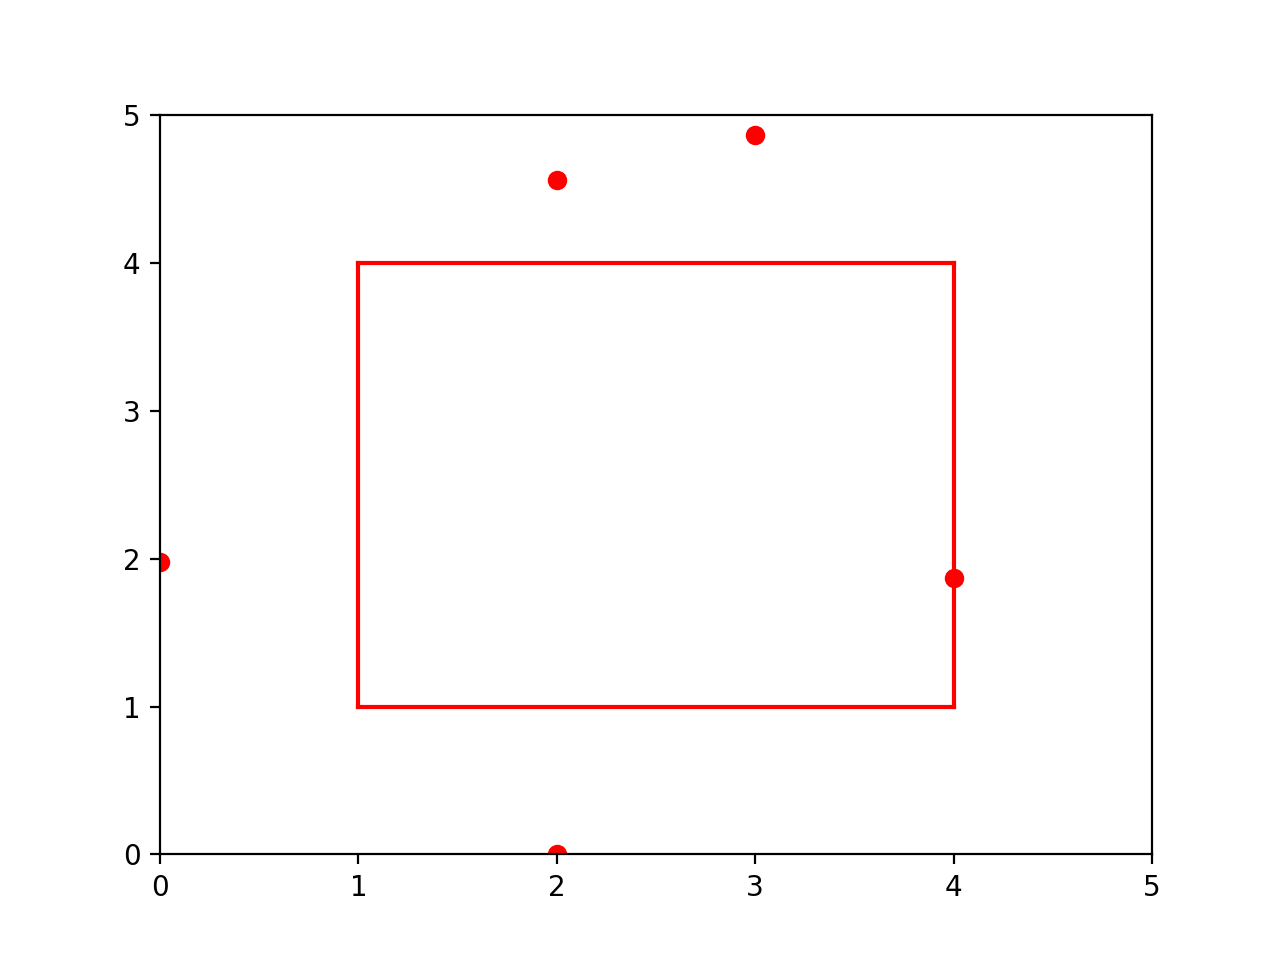
\includegraphics[width=0.5\textwidth]{Bounded_LBFGS}
    \caption{Optimal configuration of LEDs for region bounded by [1, 4] horizontally and [1, 4] vertically, yielding error value of 0.11}
    \label{bounded_solution}
\end{figure}

Our algorithm was then modified to handle a bounded target plane. While the initial optimization algorithm returned the LED configuration with the most uniform light distribution across the entire target plane, it was modified to consider input constraints on the size of the target plane. This was motivated by both convenience, since a bounded region would better demonstrate the functionality of our system, but also by practicality, since most applications of light optimization are concerned with uniformly lighting central areas of the room more so than the corners. As such, our modified algorithm takes additional inputs -- left, right, lower, and upper bounds -- and determines the LED configuration which achieves maximally uniform light distribution within the bounded zone. The same optimization routine as above was used, and tested on the same sample case with horizontal bounds $[0, 2]$ and vertical bounds $[0, 2]$ (Figure \ref{bounded_solution}).

Due to the robust nature of SciPy, our optimization framework is highly scalable and can accomodate many different types of optimization (non-convex, bounded/unbounded, integer programming, etc.). Although the objective function must be redefined based on the desired optimization goal, our system retains the ability to collect data and manipulate objects accordingly in real time, without loss of functionality.








%\section{Results}
%\section{Conclusion}


\bibliographystyle{alpha}
\medskip
 
\begin{thebibliography}{2}

\bibitem{su} 
Z. Su, D. Xue, and Z. Ji, "Designing LED array for uniform illumination distribution by simulated annealing algorithm," Opt. Express \textbf{20}(23), 843–855 (2012).

\bibitem{moreno} 
I. Moreno, J. Muñoz, and R. Ivanov, “Uniform illumination of distant targets using a spherical light-emitting diode array,” Opt. Eng. \textbf{46}(3), 033001 (2007).

\end{thebibliography}


\end{document}






